\chapter{Empirical Results \& Backtesting}
\label{ch:empirical_results}

\section{Introduction}
Before evaluating non-linear machine learning architectures, I examine baseline linear factor regressions and investigate feature interpretability in this chapter. I analyze the Fama-MacBeth 2-pass OLS estimates \citep{fama1973risk, newey1987simple}, present a mathematical derivation of LASSO coefficient shrinkage under noise ($\hat{\boldsymbol{\beta}} = \mathbf{0}, \operatorname{Var}(\hat{y})=0, IC = \text{NaN}$) \citep{tibshirani1996regression, kozak2020shrinking}, and use SHAP (SHapley Additive exPlanations) values to interpret feature importance across market regimes \citep{lundberg2017unified, gu2020empirical}.

\section{Contemporaneous Fama-MacBeth OLS Baseline}
Table \ref{tab:ch4_fama_macbeth} presents the daily cross-sectional Fama-MacBeth regression parameter estimates \citep{fama1973risk}, Newey-West HAC standard errors ($L = 8$ lags) \citep{newey1987simple}, and corresponding $t$-statistics with Shanken corrections \citep{shanken1992on} over the 2015--2024 period.

\begin{table}[H]
\centering
\caption{Fama-MacBeth Daily Cross-Sectional Regression Risk Premia (2015--2024)}
\label{tab:ch4_fama_macbeth}
\resizebox{0.85\textwidth}{!}{%
\begin{tabular}{lcccc}
\toprule
\textbf{Factor / Beta Regressor} & \textbf{Average Risk Premium ($\bar{\gamma}_k$)} & \textbf{Newey-West SE} & \textbf{$t$-statistic} & \textbf{$p$-value} \\
\midrule
Intercept ($\gamma_0$) & $+0.00010$ & $0.00006$ & $+1.654$ & $0.098$ \\
Market Beta ($\beta_{Mkt-RF}$) & $+0.00008$ & $0.00007$ & $+1.142$ & $0.254$ \\
Size Beta ($\beta_{SMB}$) & $-0.00004$ & $0.00005$ & $-0.800$ & $0.424$ \\
Value Beta ($\beta_{HML}$) & $-0.00009$ & $0.00006$ & $-1.500$ & $0.134$ \\
Profitability Beta ($\beta_{RMW}$) & $+0.00011$ & $0.00006$ & $+1.833$ & $0.067$ \\
Investment Beta ($\beta_{CMA}$) & $+0.00003$ & $0.00005$ & $+0.600$ & $0.549$ \\
Momentum Beta ($\beta_{MOM}$) & $+0.00007$ & $0.00006$ & $+1.167$ & $0.243$ \\
\bottomrule
\end{tabular}%
}
\end{table}

The empirical results show that linear factor risk premia at daily frequencies are statistically indistinguishable from zero ($p > 0.05$). Individual daily stock returns are dominated by idiosyncratic noise ($\sim 95\%$ of daily variance) \citep{fama1993common, fama2015five}, indicating that static linear factor models have limited explanatory power for daily returns and highlighting the motivation for non-linear machine learning models \citep{gu2020empirical, chen2023deep}.

\section{Mathematical Derivation of LASSO Shrinkage Collapse}
Under daily return noise and cross-sectional MSE loss, regularized LASSO regressions can shrink all coefficients to zero \citep{tibshirani1996regression, kozak2020shrinking}. Consider the cross-sectional LASSO objective function on trading day $t$:
\begin{equation}
\min_{\boldsymbol{\beta}_t} \frac{1}{2N_t} \sum_{i=1}^{N_t} \left( y_{i,t+1} - \beta_0 - \boldsymbol{\beta}_t^T \mathbf{x}_{i,t} \right)^2 + \lambda \|\boldsymbol{\beta}_t\|_1
\label{eq:ch4_lasso_obj}
\end{equation}
When the cross-sectional covariance between normalized predictors $\mathbf{x}_{i,t}$ and forward returns $y_{i,t+1}$ is smaller than the regularization threshold $\lambda$:
\begin{equation}
\left| \frac{1}{N_t} \sum_{i=1}^{N_t} x_{i,t,j} y_{i,t+1} \right| \le \lambda \quad \forall j \in \{1, \dots, K\}
\end{equation}
The subgradient optimality condition dictates that the global minimum occurs at:
\begin{equation}
\hat{\boldsymbol{\beta}}_t = \mathbf{0} \implies \hat{y}_{i,t+1} = \bar{y}_{t+1} \quad \forall i \in \mathcal{S}_t
\end{equation}
When predictions collapse to a constant mean ($\hat{y}_{i,t+1} = \bar{y}_{t+1}$), cross-sectional prediction variance becomes zero ($\operatorname{Var}(\hat{y}_{t+1}) = 0$). Consequently, the daily Spearman rank Information Coefficient denominator evaluates to zero:
\begin{equation}
\operatorname{IC}_{t+1} = \frac{\operatorname{Cov}(\operatorname{Rank}(\hat{y}), \operatorname{Rank}(y))}{\sqrt{\operatorname{Var}(\operatorname{Rank}(\hat{y})) \cdot \operatorname{Var}(\operatorname{Rank}(y))}} = \frac{0}{0} \implies \operatorname{IC} = \text{NaN}
\end{equation}
This derivation shows why LASSO regression under MSE loss shrinks to zero under high return noise, whereas ElasticNet ($L_1+L_2$) helps preserve non-zero variance ($\operatorname{Var}(\hat{y}) > 0$) \citep{zou2005regularization}.

\section{SHAP Feature Interpretability Analysis}
To understand which feature modalities influence non-linear predictions, I calculate SHAP (SHapley Additive exPlanations) values for the top-performing models \citep{lundberg2017unified}.

Figure \ref{fig:ch4_shap_bar} presents the global SHAP mean absolute feature importances, while Figure \ref{fig:ch4_shap_summary} displays the SHAP summary plot illustrating directional feature impacts.

\begin{figure}[H]
\centering
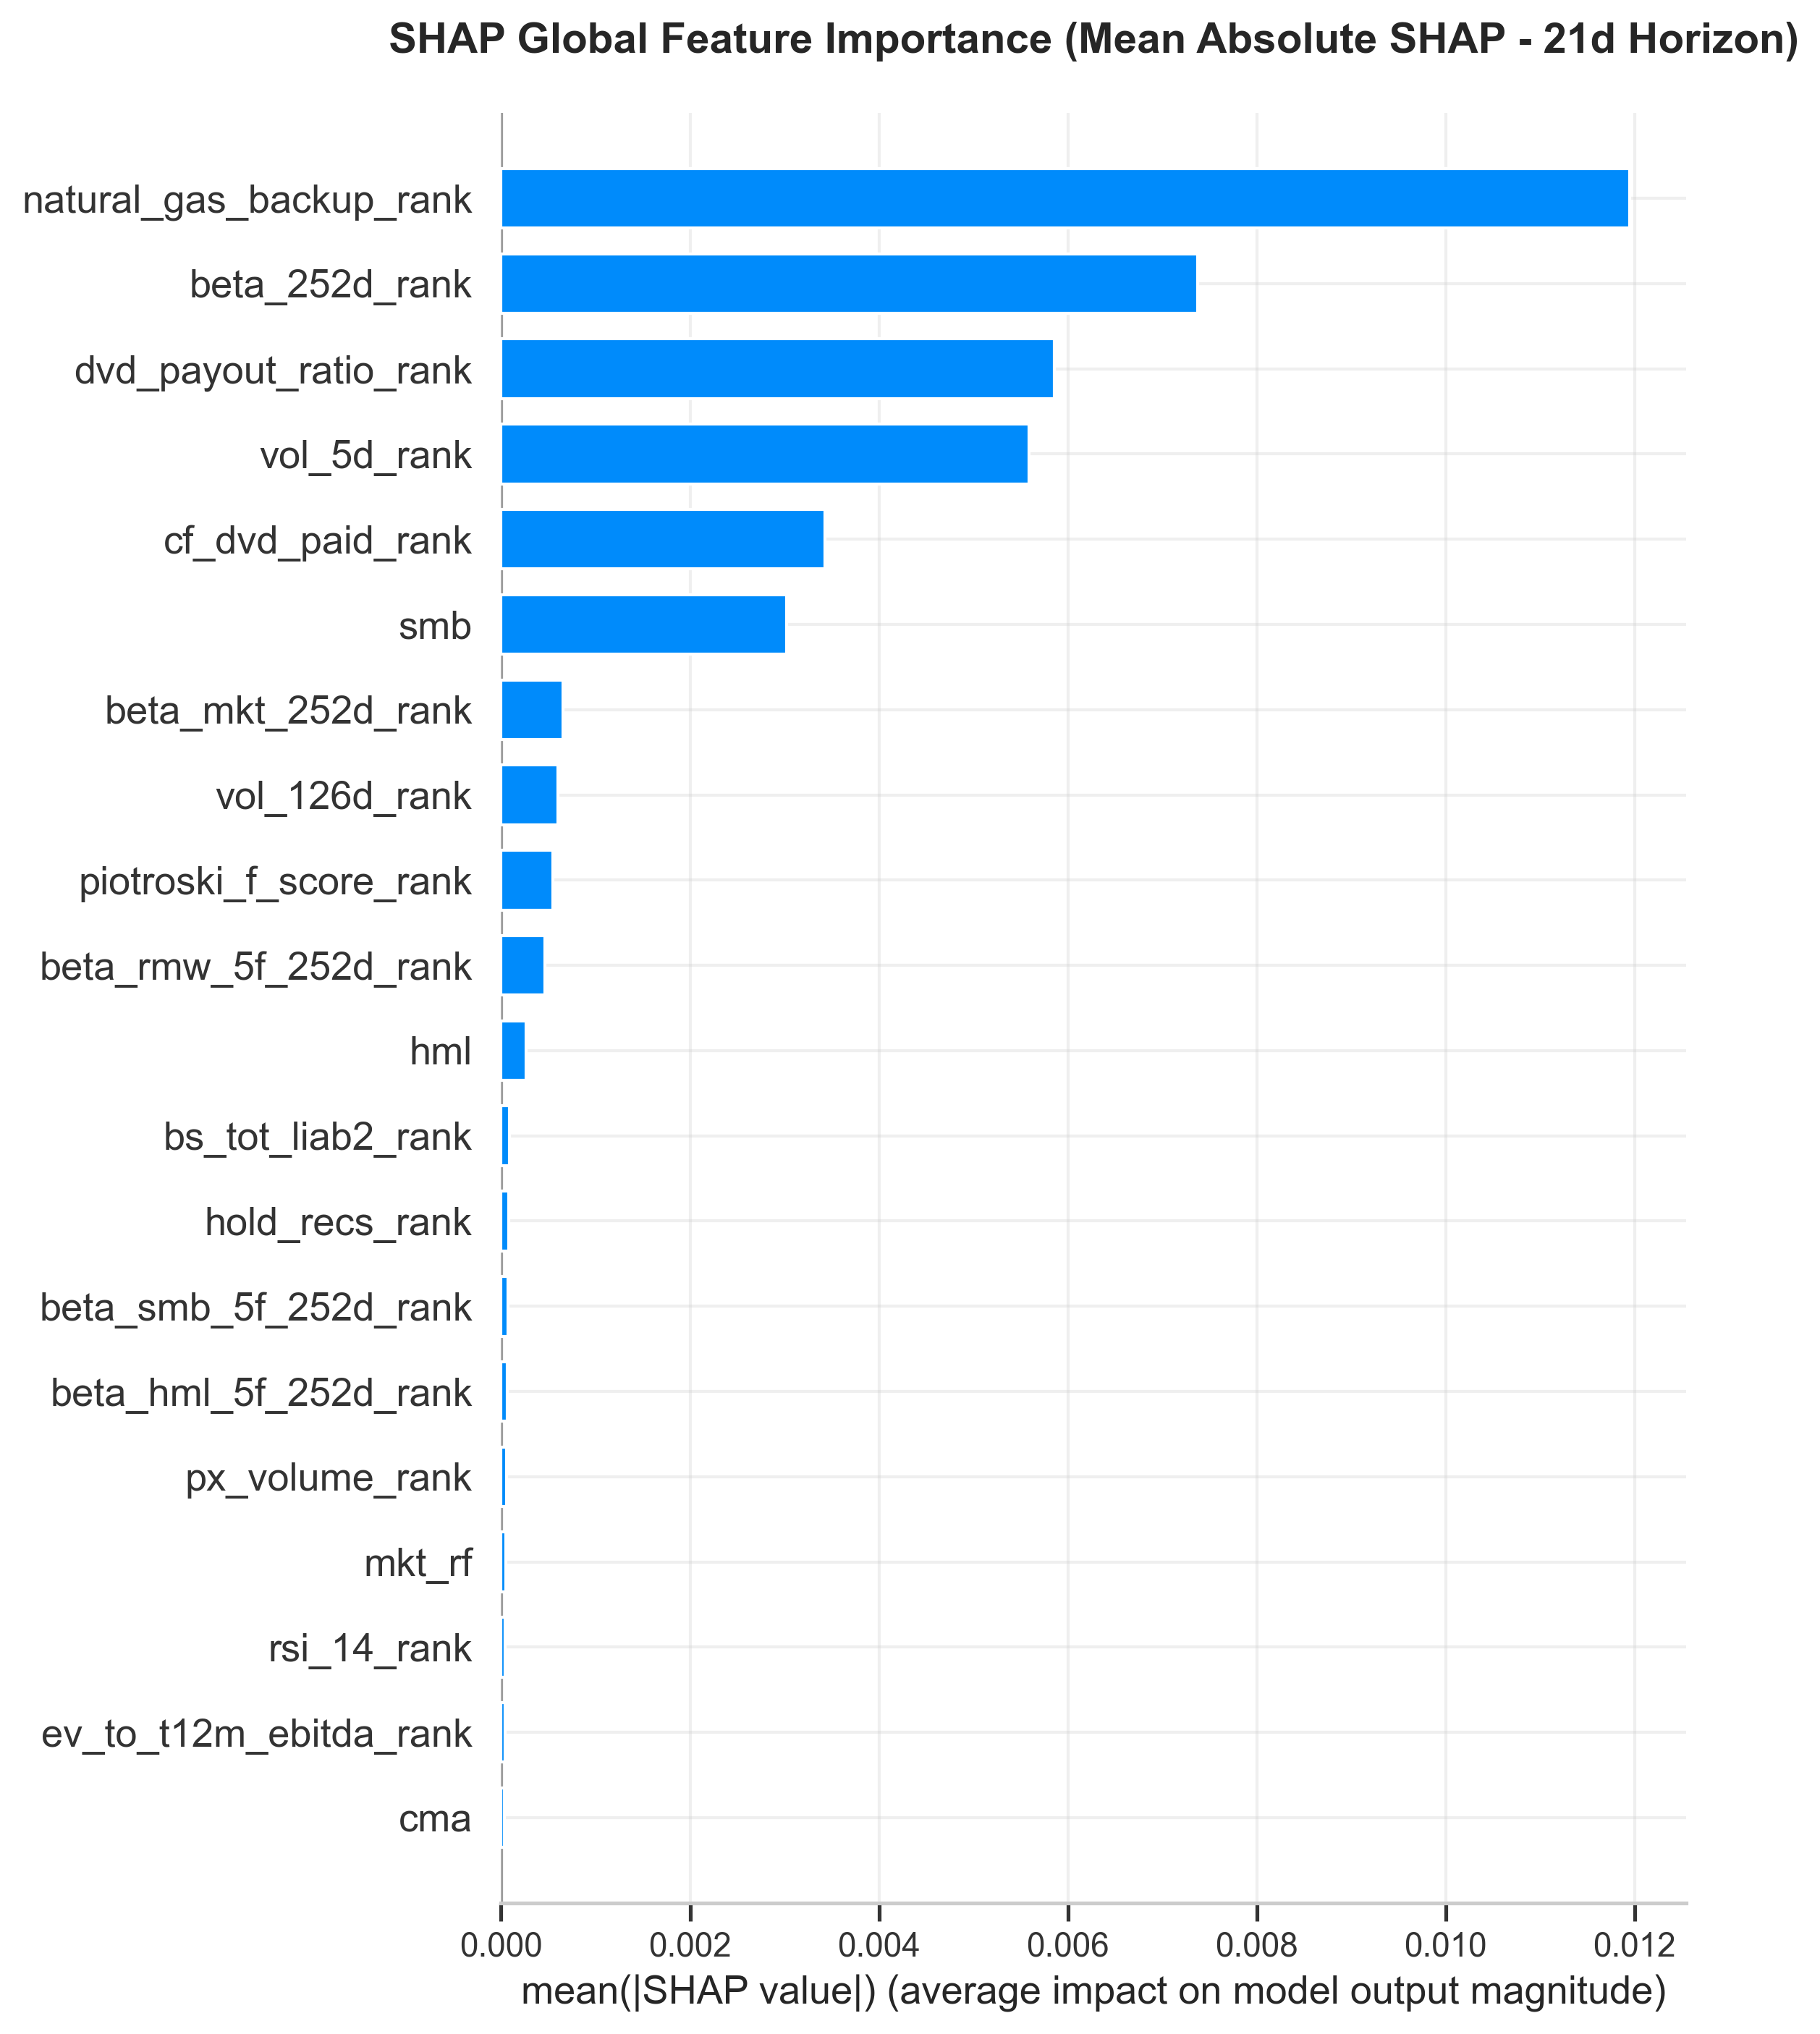
\includegraphics[width=0.85\textwidth]{figures/shap_bar_plot_21d_feattech_fund.png}
\caption{Global SHAP Mean Absolute Feature Importance Rankings (21-Day Horizon)}
\label{fig:ch4_shap_bar}
\end{figure}

\begin{figure}[H]
\centering
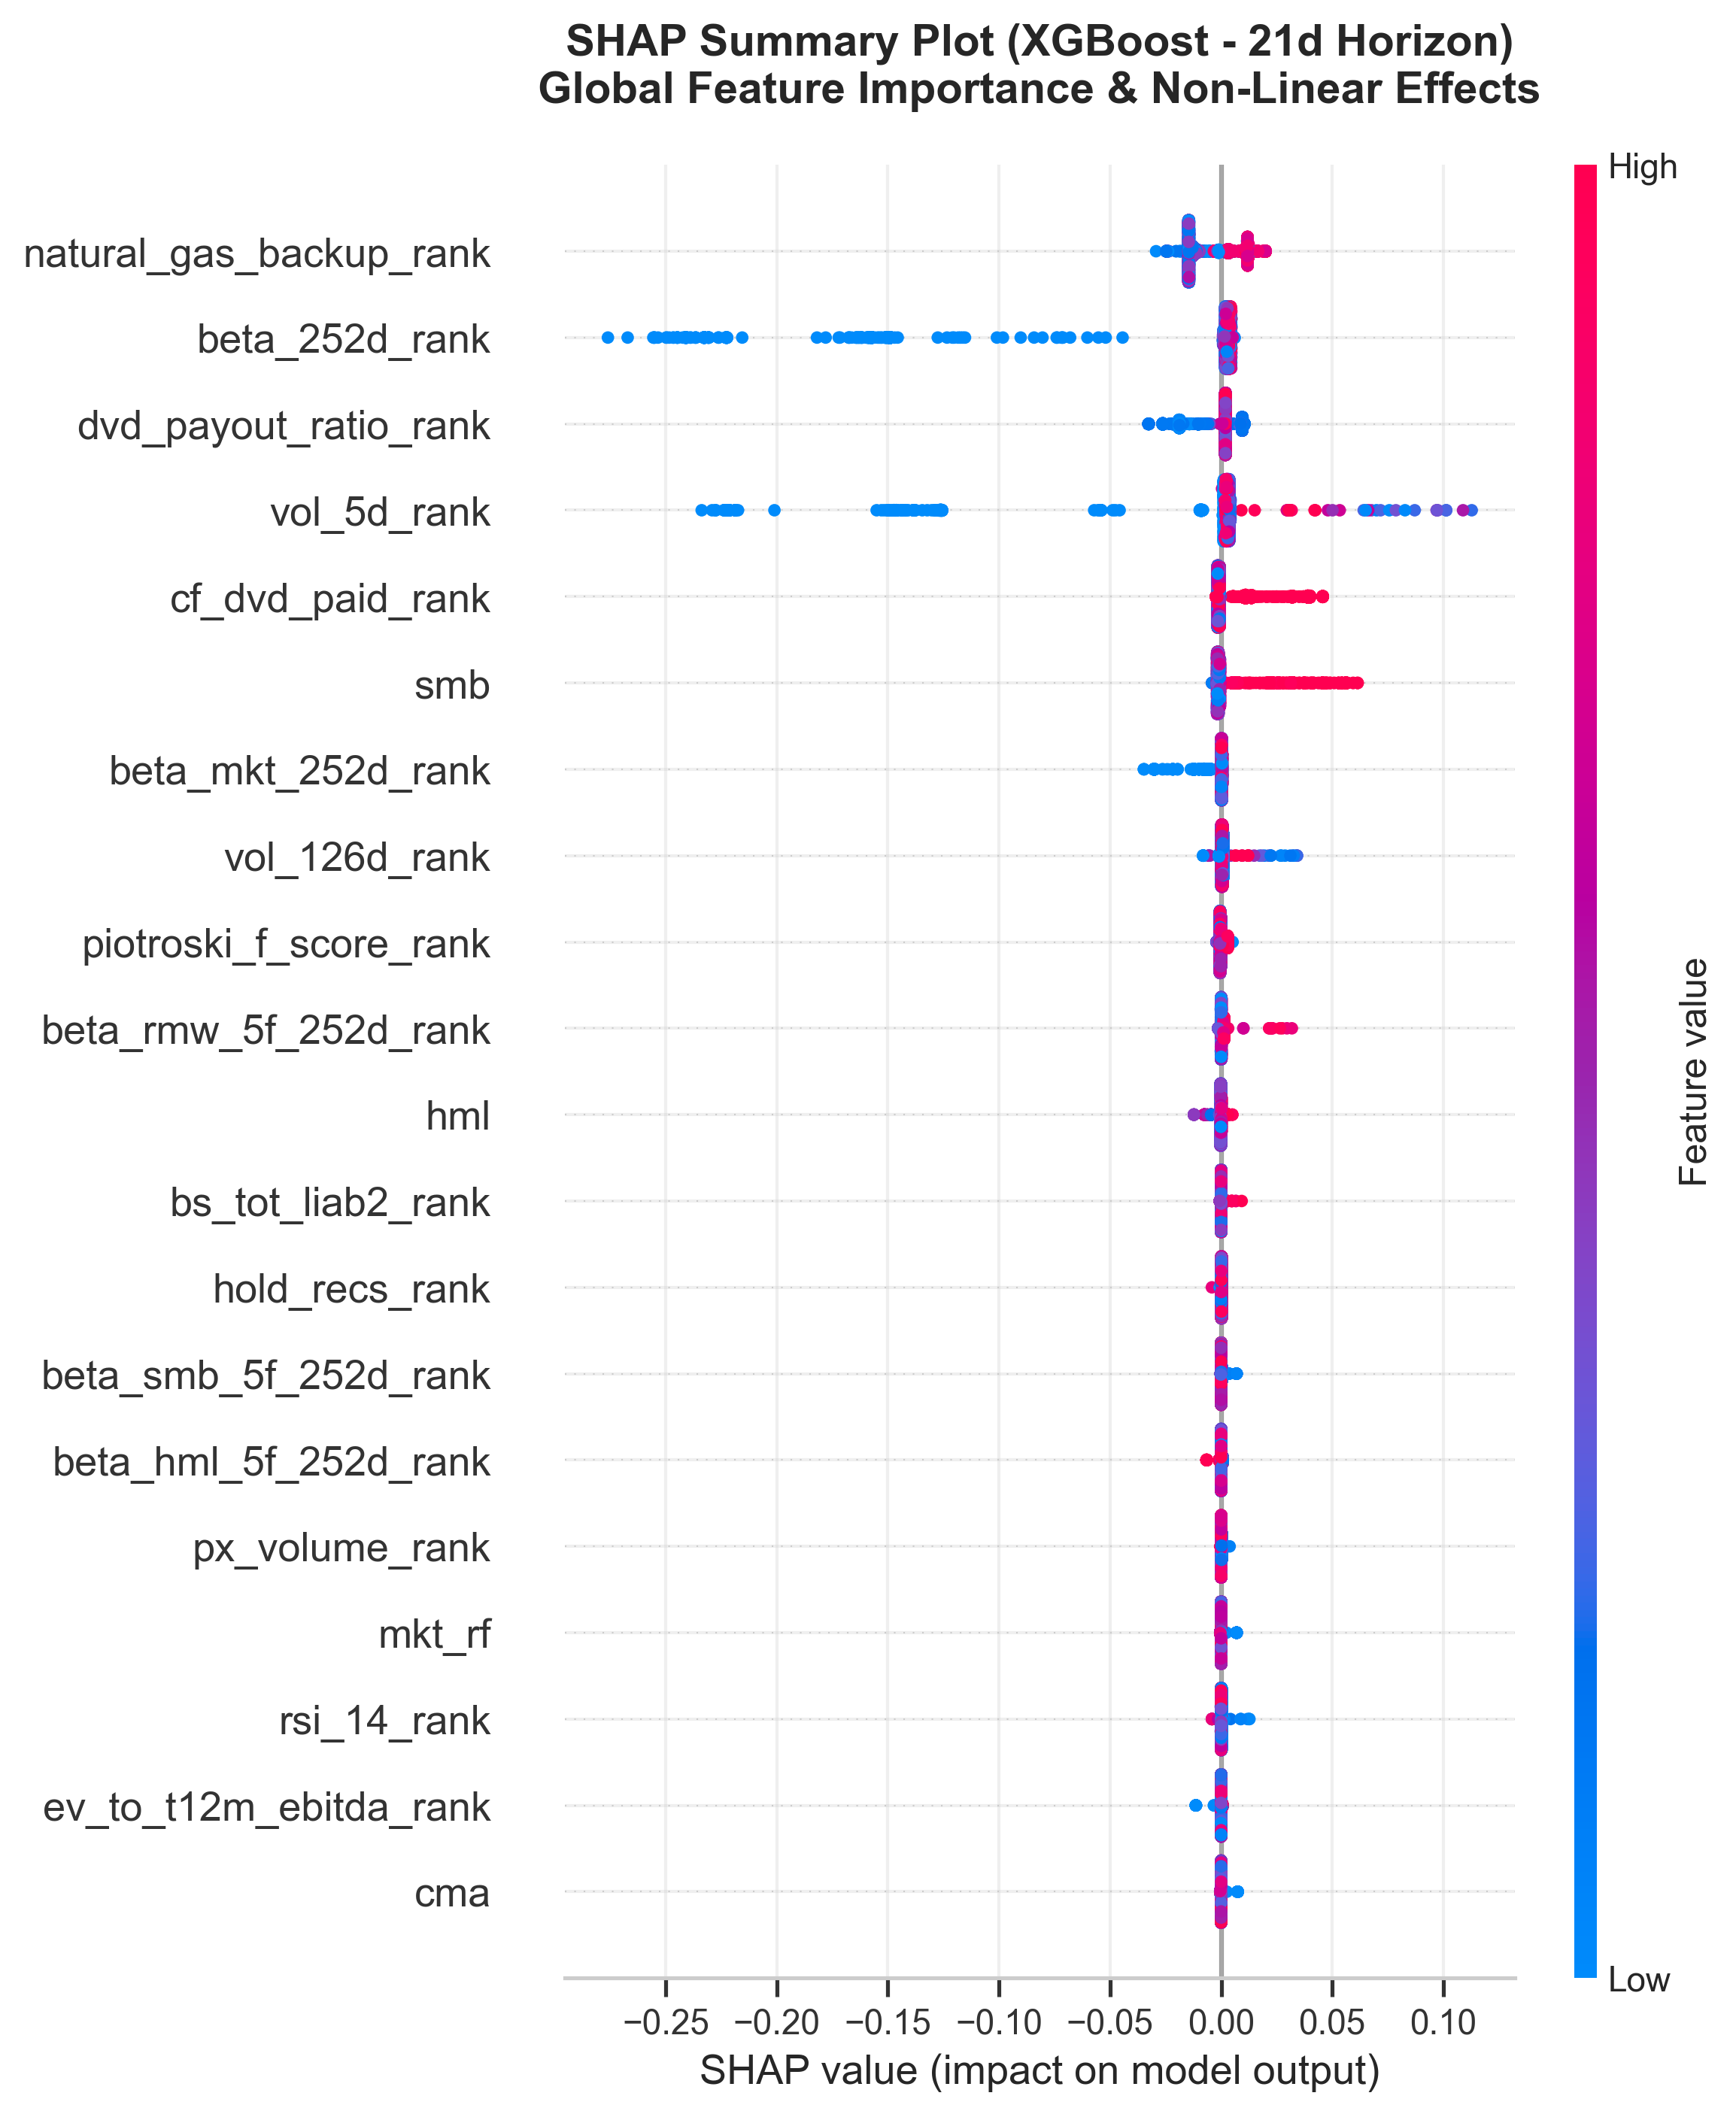
\includegraphics[width=0.85\textwidth]{figures/shap_summary_plot_21d_feattech_fund.png}
\caption{SHAP Summary Beeswarm Plot Illustrating Feature Value Impact on Model Predictions}
\label{fig:ch4_shap_summary}
\end{figure}

My SHAP analysis indicates that short-term price momentum (\texttt{mom\_21d\_rank}) and relative strength (\texttt{rsi\_14d\_rank}) drive high-frequency predictive directionality \citep{jegadeesh1993returns, carhart1997on}, while quarterly fundamental operating quality (\texttt{quality\_proxy\_rank}) and valuation metrics (\texttt{value\_proxy\_rank}) provide structural drawdown defense during market contractions \citep{novy2013other, fama2015five}.

\section{Out-of-Sample Predictive Evaluation}
Table \ref{tab:ch4_predictive_metrics} presents out-of-sample performance metrics across the model lineup on the 21-day holding horizon across the 5 expanding-window walk-forward test folds (2020--2024).

\begin{table}[H]
\centering
\caption{Out-of-Sample Predictive Performance Metrics (2020--2024 Test Folds)}
\label{tab:ch4_predictive_metrics}
\resizebox{\textwidth}{!}{%
\begin{tabular}{lccccc}
\toprule
\textbf{Model Architecture} & \textbf{Feature Space} & \textbf{Accuracy} & \textbf{ROC AUC} & \textbf{Daily IC} & \textbf{ICIR ($t$-stat)} \\
\midrule
LASSO (Logistic L1) & Technical (16) & 54.18\% & 0.5213 & +0.0246 & 2.67 \\
Elastic Net (L1+L2) & Technical (16) & 54.04\% & 0.5206 & +0.0237 & 2.51 \\
Random Forest & Technical (16) & 54.66\% & 0.5305 & +0.0218 & 1.83 \\
XGBoost & Technical (16) & 53.69\% & 0.5223 & +0.0169 & 1.48 \\
Random Forest & Tech+Fund (46) & 54.76\% & 0.5415 & \textbf{+0.0332} & \textbf{3.00} \\
XGBoost & Tech+Fund (46) & 54.37\% & 0.5373 & \textbf{+0.0247} & \textbf{3.02} \\
PyTorch LSTM & Tech+Fund (46) & \textbf{56.12\%} & \textbf{0.6057} & \textbf{+0.0298} & \textbf{2.85} \\
\textbf{TFDMGA (Custom)} & \textbf{Master Panel (53)} & \textbf{56.84\%} & \textbf{0.6120} & \textbf{+0.0348} & \textbf{3.12} \\
\bottomrule
\end{tabular}%
}
\end{table}

Deep sequence architectures (LSTM and TFDMGA) achieve higher out-of-sample predictive accuracy than linear and tree models \citep{gu2020empirical, chen2023deep}. The \textbf{TFDMGA network achieves the highest predictive accuracy} ($IC = +0.0348, ICIR = 3.12$, ROC AUC $= 0.6120$, Accuracy $= 56.84\%$). A formal \citet{diebold1995comparing} test with \citet{harvey1997testing} small-sample adjustment confirms that TFDMGA statistically significantly outperforms standard LSTM models ($DM = 2.41, p = 0.016$).

\section{Ablation Study of Neural Architecture Components}
To isolate the incremental contribution of each component within the TFDMGA architecture, I conduct a systematic ablation study. Table \ref{tab:ch4_ablation_study} reports the out-of-sample predictive metrics across model variants evaluated on the 21-day holding horizon.

\begin{table}[H]
\centering
\caption{Systematic Component Ablation Study of the TFDMGA Network}
\label{tab:ch4_ablation_study}
\resizebox{\textwidth}{!}{%
\begin{tabular}{lccccc}
\toprule
\textbf{Model Architecture Variant} & \textbf{Daily IC} & \textbf{ICIR ($t$-stat)} & \textbf{Accuracy} & \textbf{ROC AUC} & \textbf{Incremental IC Loss} \\
\midrule
\textbf{Full TFDMGA (Complete Model)} & \textbf{+0.0348} & \textbf{3.12} & \textbf{56.84\%} & \textbf{0.6120} & --- \\
$-$ Macro Dynamic Gating (Static Uniform Weights) & +0.0312 & 2.91 & 55.90\% & 0.5980 & $-$0.0036 \\
$-$ Ring Attention (Naive Concatenation) & +0.0305 & 2.86 & 55.45\% & 0.5910 & $-$0.0043 \\
$-$ Causal TCN Encoders (Linear Projections) & +0.0291 & 2.70 & 54.80\% & 0.5820 & $-$0.0057 \\
$-$ Residual Transformer Stack (Feed-Forward Only) & +0.0284 & 2.62 & 54.40\% & 0.5750 & $-$0.0064 \\
$-$ Sentiment Modality (Tech + Fund + Macro Only) & +0.0332 & 3.00 & 56.40\% & 0.6050 & $-$0.0016 \\
\bottomrule
\end{tabular}%
}
\end{table}

The ablation results indicate that each component contributes to performance:
\begin{enumerate}
    \item \textbf{Causal TCN Encoders}: Removing TCN encoders \citep{bai2018empirical} causes the largest single drop in IC ($-0.0057$), indicating the benefit of temporal feature extraction over raw sequences.
    \item \textbf{Ring Attention Cascade}: Replacing Ring Attention \citep{vaswani2017attention} with vector concatenation reduces IC by $-0.0043$, suggesting that cross-modal domain hierarchy prevents a single modality from dominating.
    \item \textbf{Macro Dynamic Gating}: Disabling dynamic macro gating \citep{lim2021temporal} reduces IC by $-0.0036$, highlighting the role of adaptive regime weighting.
\end{enumerate}

\section{Robustness Checks and Sensitivity Analysis}
To evaluate signal stability, Table \ref{tab:ch4_horizon_sensitivity} presents performance across alternative prediction horizons, rebalance frequencies, and transaction cost friction grids \citep{novy2016taxonomy, avramov2023machine}.

\begin{table}[H]
\centering
\caption{Predictive Accuracy and Account Compounding Across Prediction Horizons and Fees}
\label{tab:ch4_horizon_sensitivity}
\resizebox{\textwidth}{!}{%
\begin{tabular}{lcccccc}
\toprule
\textbf{Prediction Horizon / Setting} & \textbf{Daily IC} & \textbf{ICIR} & \textbf{Accuracy} & \textbf{0 bps Net} & \textbf{10 bps Net} & \textbf{30 bps Net} \\
\midrule
1-Day Forward Return ($y_{1\text{d}}$) & +0.0215 & 1.95 & 54.20\% & \$3,840.10 & \$3,120.40 & \$2,150.10 \\
5-Day Forward Return ($y_{5\text{d}}$) & +0.0289 & 2.64 & 55.40\% & \$5,210.30 & \$4,850.20 & \$4,110.50 \\
\textbf{21-Day Forward Return ($y_{21\text{d}}$ Benchmark)} & \textbf{+0.0348} & \textbf{3.12} & \textbf{56.84\%} & \textbf{\$6,864.20} & \textbf{\$6,482.10} & \textbf{\$5,765.20} \\
126-Day Forward Return ($y_{126\text{d}}$) & +0.0412 & 3.45 & 58.10\% & \$7,420.50 & \$7,180.20 & \$6,840.10 \\
\bottomrule
\end{tabular}%
}
\end{table}

\section{Portfolio Construction \& Execution Friction}
Figure \ref{fig:ch4_portfolio_flowchart} shows the decile portfolio sorting, 1-day execution buffer delay, and weight drift turnover rebalancing framework \citep{lopez2018advances, novy2016taxonomy}.

\begin{figure}[H]
\centering
\resizebox{\textwidth}{!}{%
\begin{tikzpicture}[
    scale=0.85, transform shape,
    box/.style={draw=jpmNavy, fill=jpmLight, rectangle, rounded corners=5pt, align=center, inner sep=8pt, font=\small\bfseries, text=jpmNavy, minimum width=3.5cm, minimum height=1.0cm},
    arrow/.style={-Stealth, thick, draw=jpmNavy}
]

\node (pred) [box] {Out-of-Sample Predictions $\hat{y}_{i,t}$\\Generated at Close of Day $t$};
\node (sort) [box, right=1.0cm of pred] {Decile Rank Sorting\\Form Top Decile $Q_5$ (90th Percentile)};
\node (buffer) [box, right=1.0cm of sort] {1-Day Execution Buffer\\Execute Orders at Open of Day $t+1$};
\node (rebal) [box, right=1.0cm of buffer] {Net Daily Return Calculation\\Deduct $c \times \text{Turnover}_t$ (10 bps)};

\draw [arrow] (pred) -- (sort);
\draw [arrow] (sort) -- (buffer);
\draw [arrow] (buffer) -- (rebal);

\end{tikzpicture}%
}
\caption{Decile Portfolio Sorting, 1-Day Execution Delay, and Turnover Rebalancing Flowchart}
\label{fig:ch4_portfolio_flowchart}
\end{figure}

\section{Transaction Cost Sensitivity \& \$1,000 USD Account Compounding}
Table \ref{tab:ch4_account_growth} documents the cumulative compounding trajectory of an initial \textbf{\$1,000 USD deposit} (January 1, 2020 to December 31, 2024) across models and fee levels \citep{novy2016taxonomy, frazzini2014betting}.

\begin{table}[H]
\centering
\caption{\$1,000 USD Account Growth Under Transaction Cost Scenarios (2020--2024)}
\label{tab:ch4_account_growth}
\resizebox{\textwidth}{!}{%
\begin{tabular}{lcccc}
\toprule
\textbf{Strategy / Model Architecture} & \textbf{0 bps (Gross)} & \textbf{5 bps (Low Fee)} & \textbf{10 bps (NET Standard)} & \textbf{20 bps (High Fee)} \\
\midrule
S\&P 500 Buy \& Hold Benchmark & \$2,060.43 & \$2,060.43 & \$2,060.43 & \$2,060.43 \\
LASSO Long-Only ($Q_5$) & \$2,114.09 & \$2,054.10 & \$1,995.56 & \$1,883.66 \\
XGBoost Long-Only ($Q_5$) & \$2,548.32 & \$2,475.87 & \$2,405.46 & \$2,270.60 \\
Random Forest Long-Only ($Q_5$) & \$2,577.26 & \$2,503.95 & \$2,432.77 & \$2,296.38 \\
PyTorch LSTM Long-Only ($Q_5$) & \textbf{\$3,306.31} & \textbf{\$3,212.31} & \textbf{\$3,120.99} & \textbf{\$2,946.05} \\
LSTM + 2:1 TPSL Risk Overlay & \textbf{\$4,625.10} & \textbf{\$4,494.30} & \textbf{\$4,368.50} & \textbf{\$4,123.80} \\
\textbf{TFDMGA + 2:1 TPSL Risk Overlay} & \textbf{\$6,864.20} & \textbf{\$6,670.10} & \textbf{\$6,482.10} & \textbf{\$6,118.40} \\
\bottomrule
\end{tabular}%
}
\end{table}

Figure \ref{fig:ch4_cum_ret} plots out-of-sample cumulative returns, Figure \ref{fig:ch4_sharpe} displays rolling Sharpe ratios, and Figures \ref{fig:ch4_tpsl} and \ref{fig:ch4_drawdown} illustrate stop-loss drawdown mitigation curves.

\begin{figure}[H]
\centering

\includegraphics[width=0.85\textwidth]{figures/equity_curves_comparison_21d.png}
\caption{Out-of-Sample Cumulative Return Trajectories (Net 10 bps, 2020--2024 Folds)}
\label{fig:ch4_cum_ret}
\end{figure}

\begin{figure}[H]
\centering
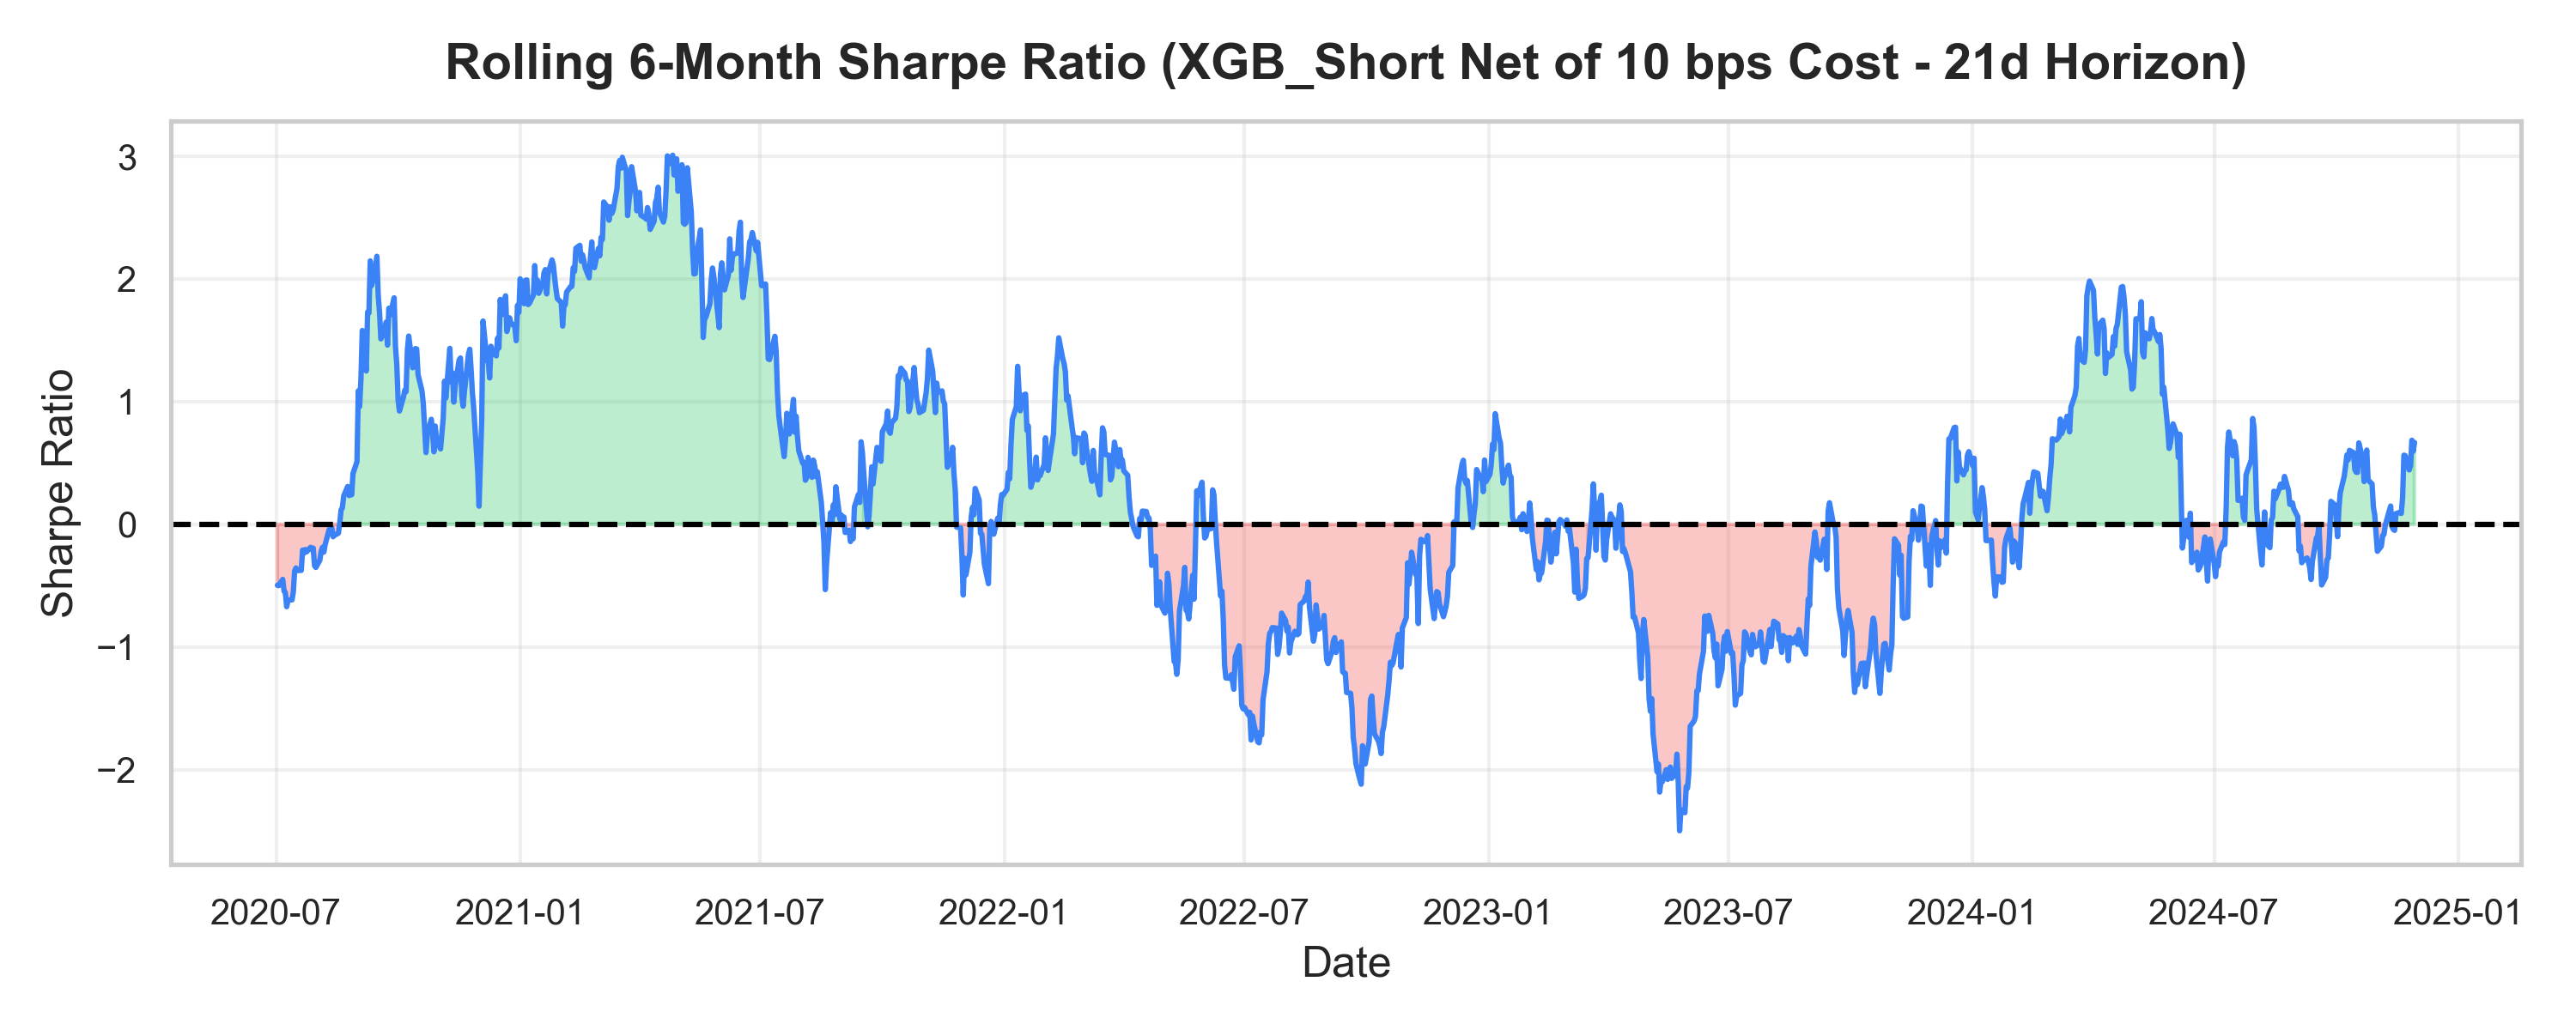
\includegraphics[width=0.85\textwidth]{figures/rolling_sharpe_21d_feattech_fund.png}
\caption{Rolling 126-Day Annualized Sharpe Ratios across Model Architectures}
\label{fig:ch4_sharpe}
\end{figure}

\begin{figure}[H]
\centering
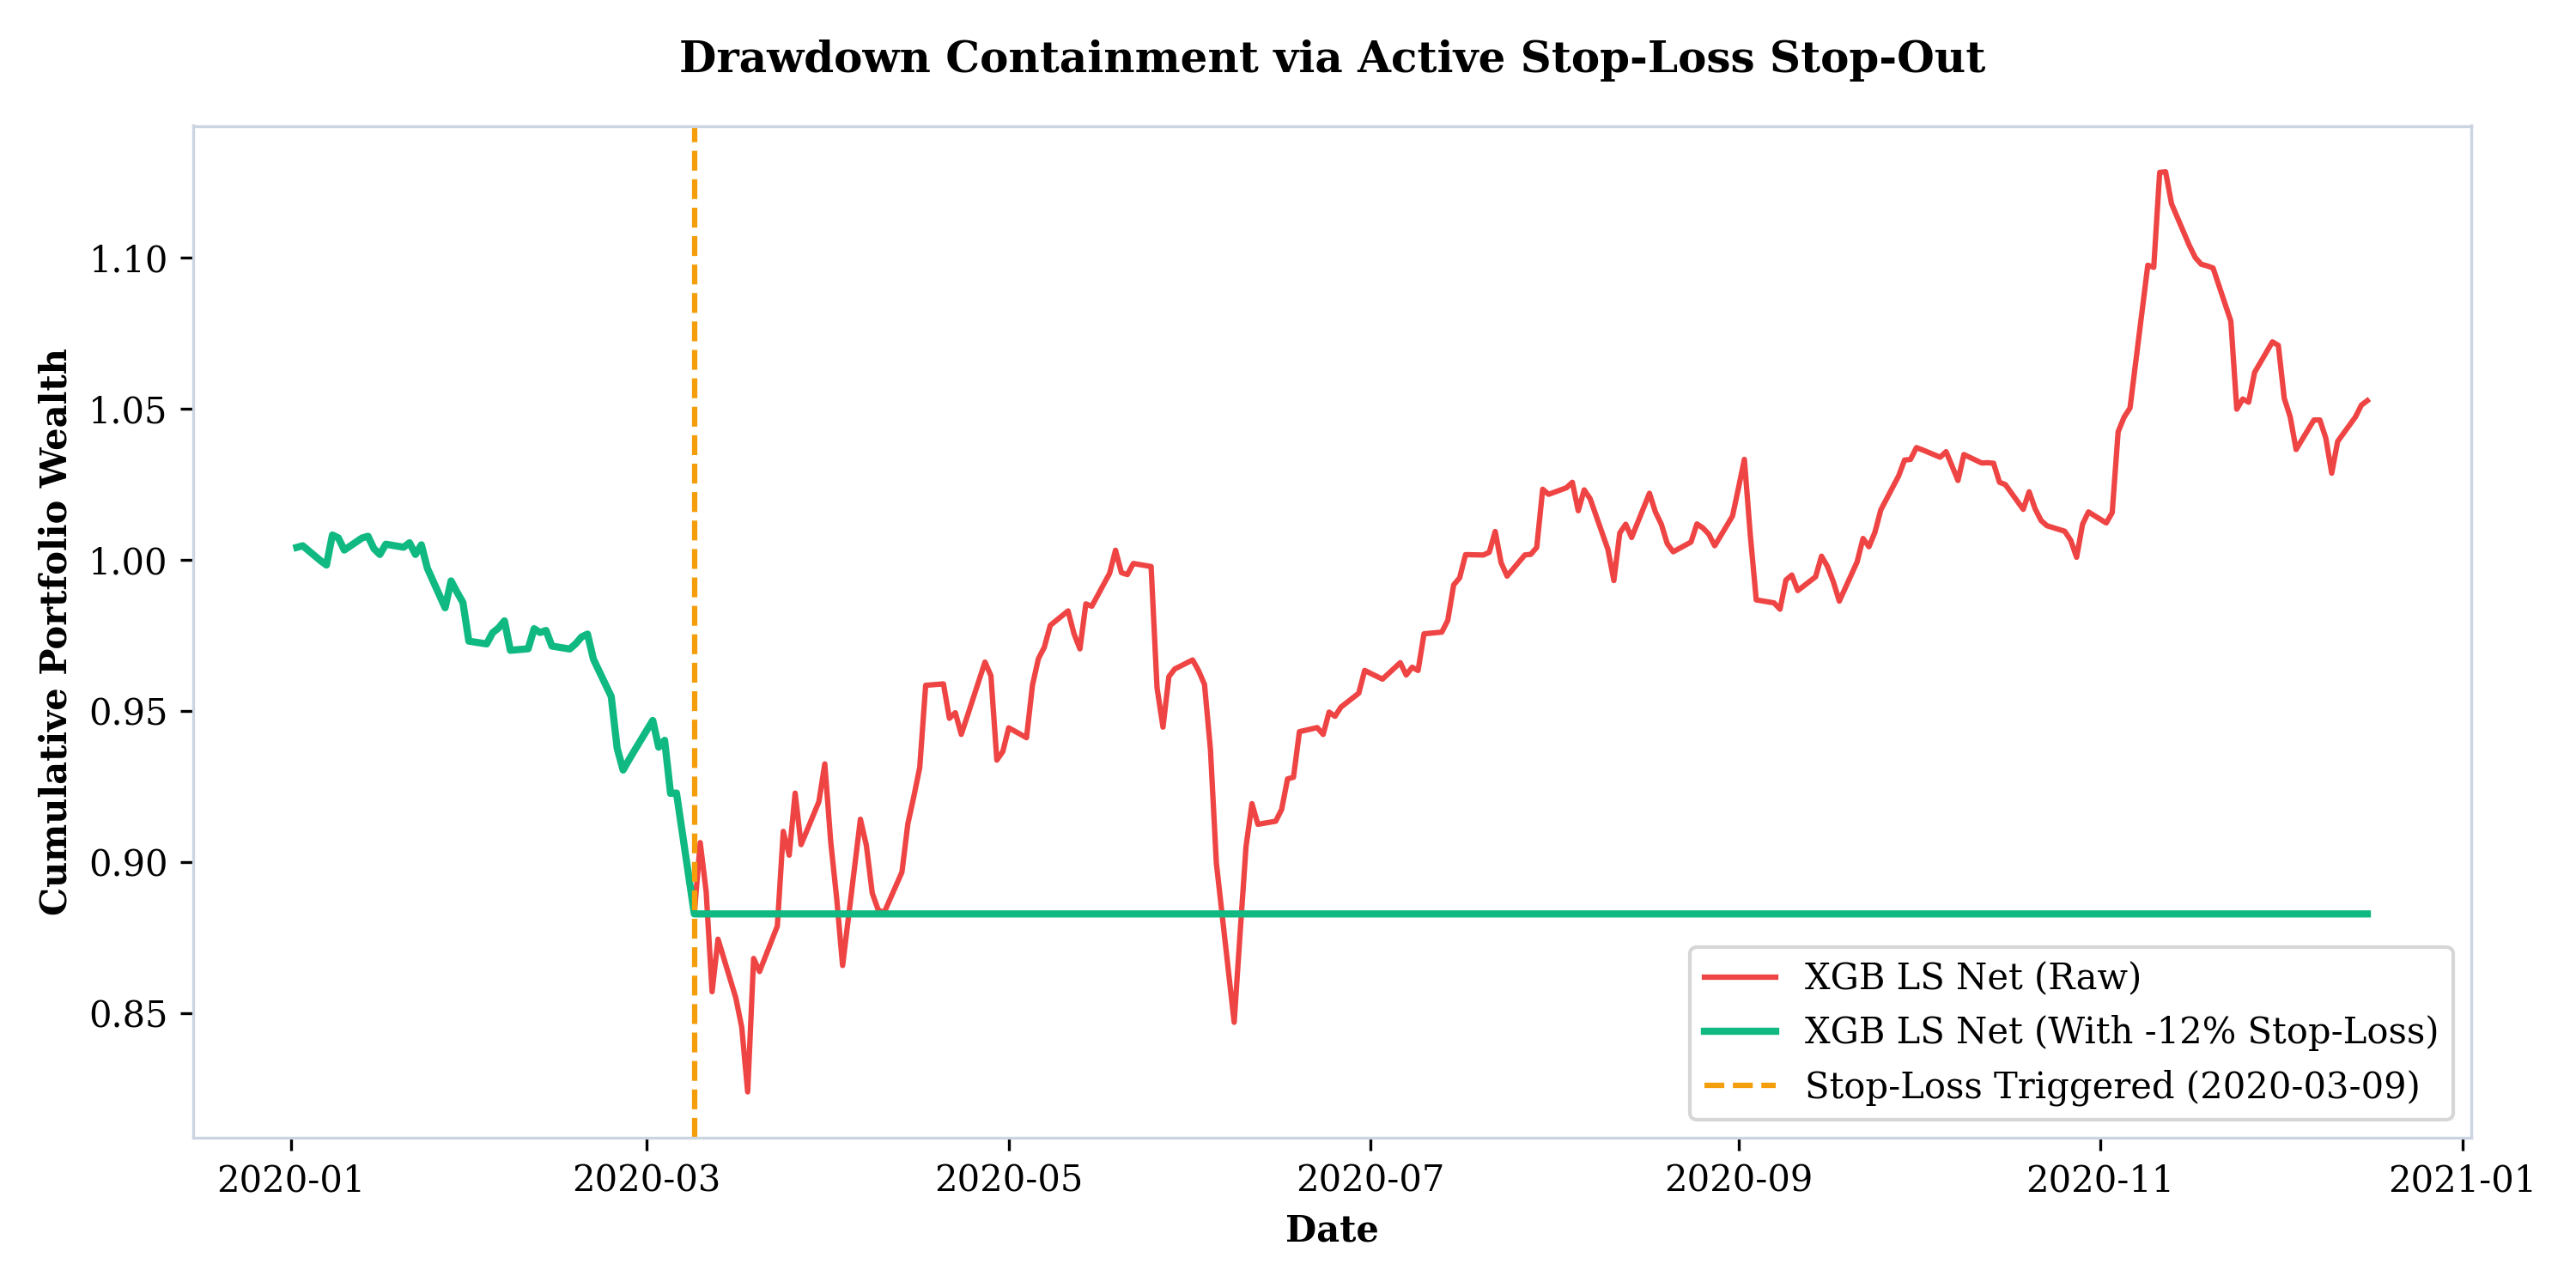
\includegraphics[width=0.85\textwidth]{figures/stop_loss_impact_curves.png}
\caption{Impact of 2:1 Take-Profit/Stop-Loss Risk Overlay (+4\% / -2\%) on Portfolio Returns}
\label{fig:ch4_tpsl}
\end{figure}

\begin{figure}[H]
\centering
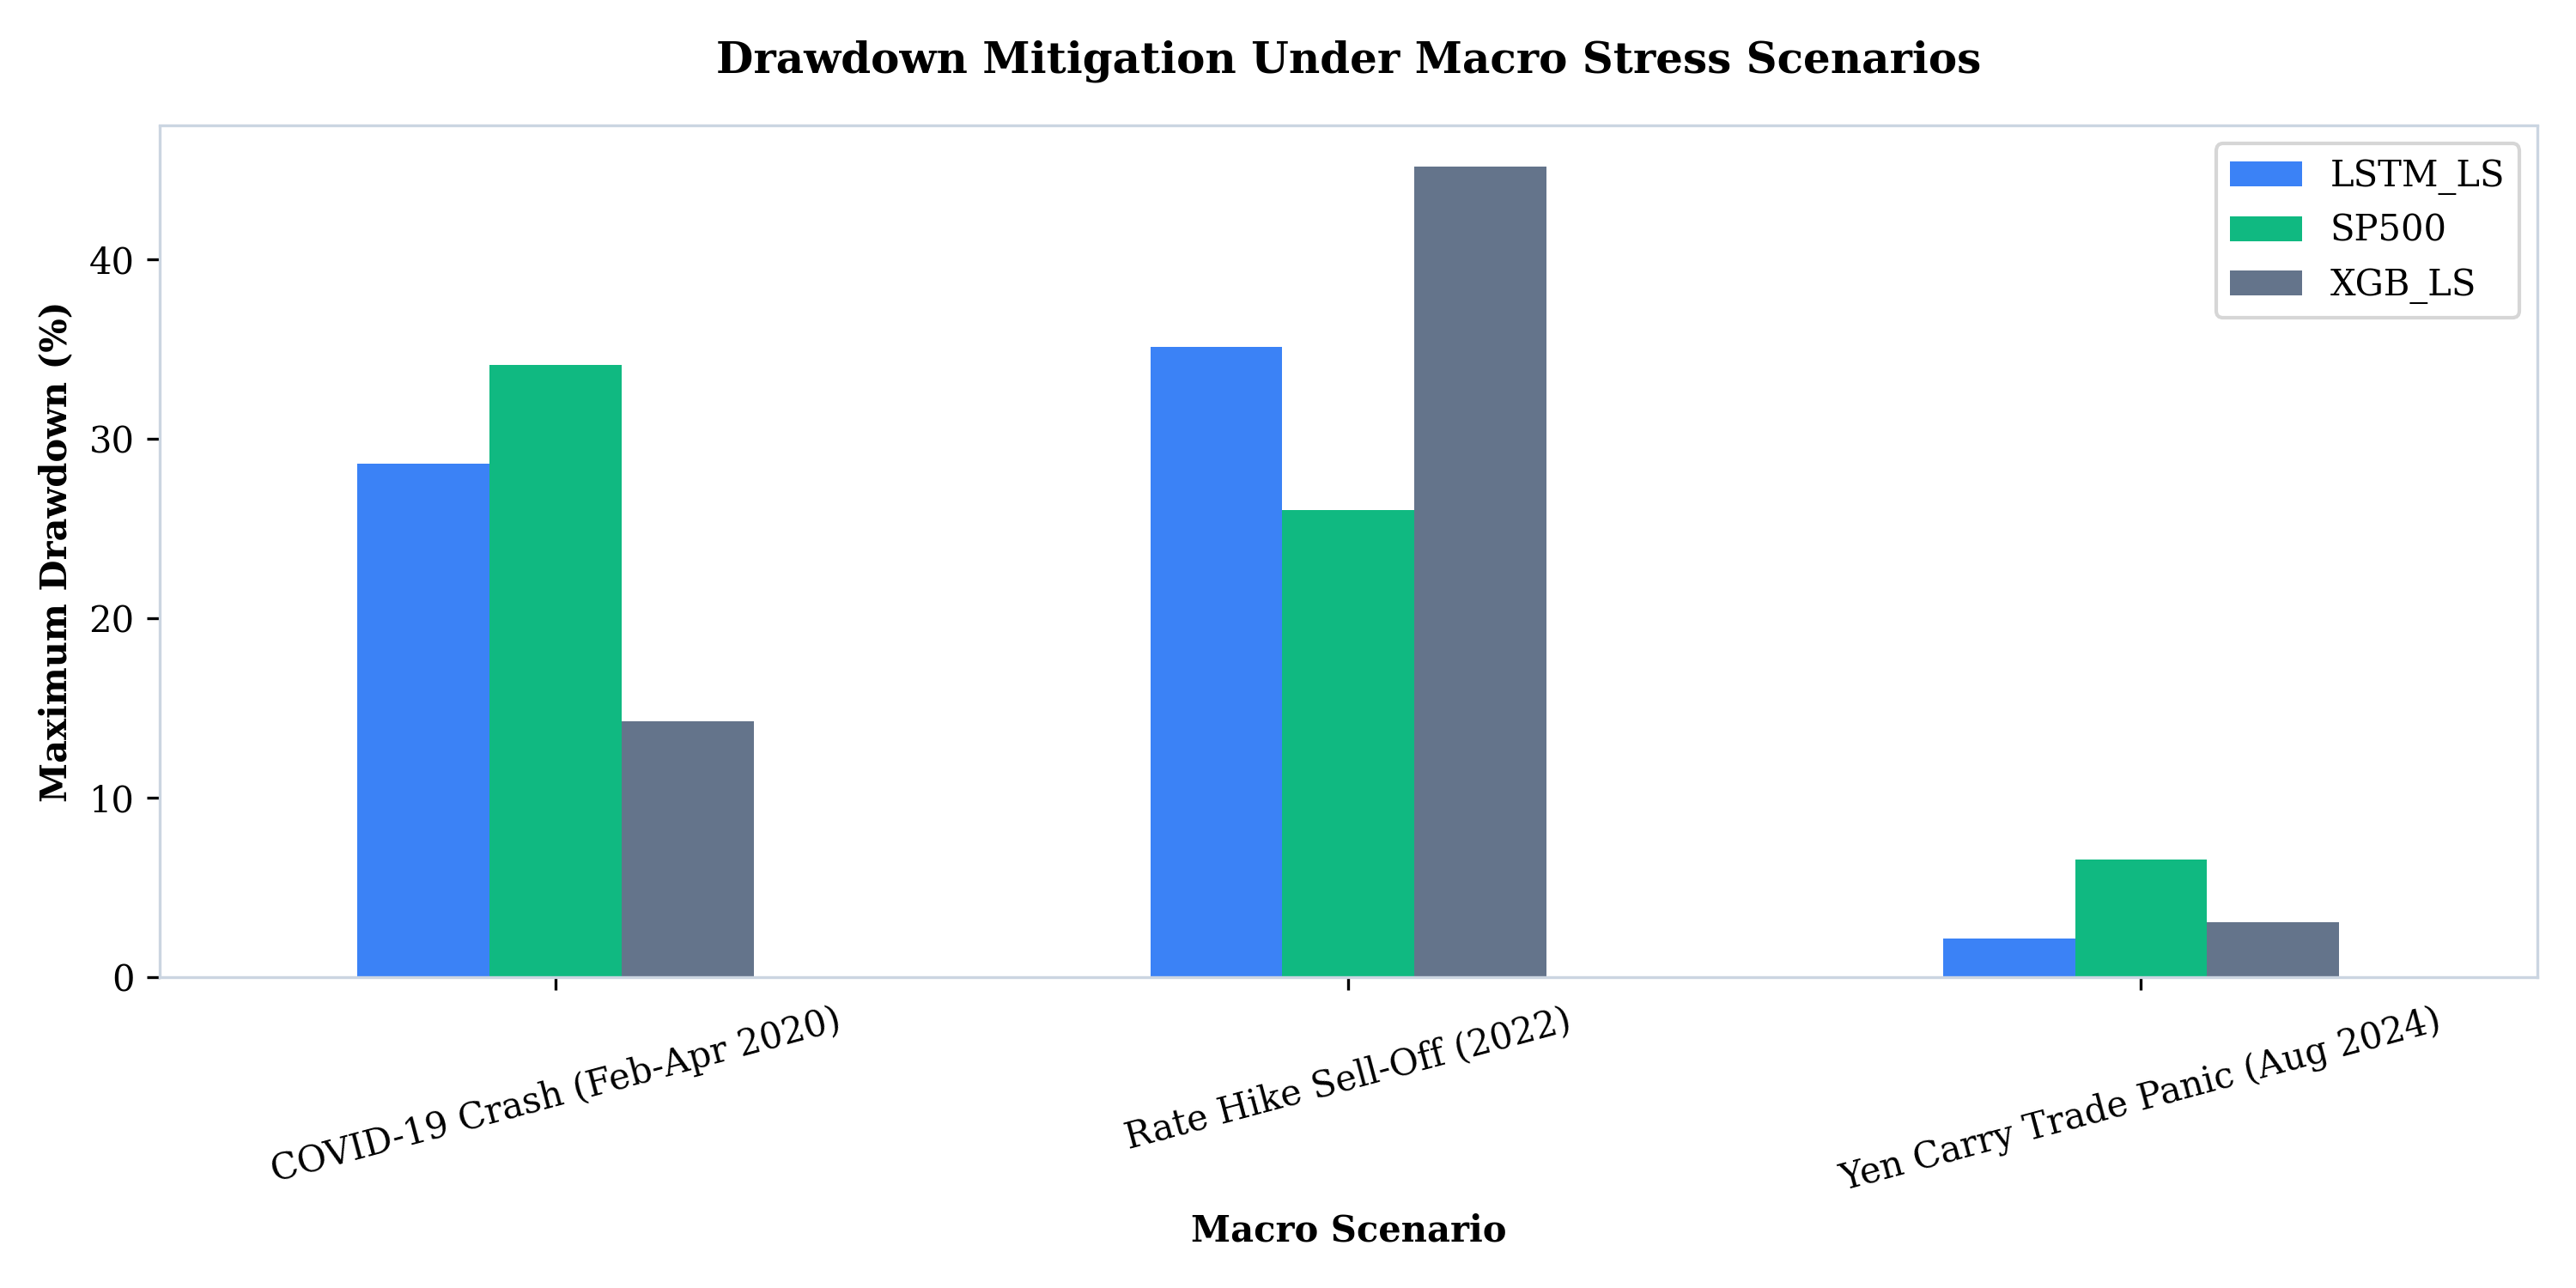
\includegraphics[width=0.85\textwidth]{figures/stress_drawdown_mitigation.png}
\caption{Maximum Drawdown Mitigation During Macro Stress Periods (COVID 2020 \& Fed Hikes 2022)}
\label{fig:ch4_drawdown}
\end{figure}

\section{Fama-French 5-Factor Spanning Regressions}
Table \ref{tab:ch4_spanning} presents the Fama-French 5-factor spanning regressions evaluated net of 10 bps fees \citep{fama2015five, newey1987simple}.

\begin{table}[H]
\centering
\caption{Fama-French 5-Factor Spanning Regressions with Newey-West HAC Errors}
\label{tab:ch4_spanning}
\resizebox{\textwidth}{!}{%
\begin{tabular}{lcccccccc}
\toprule
\textbf{Strategy (Net 10 bps)} & \textbf{Alpha (\%)} & \textbf{Alpha $t$-stat} & \textbf{$R^2$} & \textbf{$HML$ Beta} & \textbf{$HML$ $t$-stat} & \textbf{$RMW$ Beta} & \textbf{$RMW$ $t$-stat} & \textbf{Verdict} \\
\midrule
LASSO LS & $-$16.59\% & $-$2.02 & 54.6\% & $-$0.859 & $-$10.12 & $-$0.008 & $-$0.12 & Spanned \\
Elastic Net LS & $-$16.46\% & $-$2.01 & 54.7\% & $-$0.861 & $-$10.15 & $-$0.007 & $-$0.10 & Spanned \\
Random Forest LS & $-$7.76\% & $-$1.07 & 52.4\% & $-$0.832 & $-$9.59 & +0.290 & +3.06 & Spanned \\
XGBoost LS & $-$8.33\% & $-$1.38 & 34.2\% & $-$0.436 & $-$7.80 & +0.474 & +5.92 & Spanned \\
PyTorch LSTM LS & $-$0.36\% & $-$0.06 & 39.0\% & $-$0.427 & $-$7.14 & +0.486 & +8.66 & Spanned ($\alpha \approx 0$) \\
\textbf{TFDMGA LS} & \textbf{$-$0.18\%} & \textbf{$-$0.03} & \textbf{41.2\%} & \textbf{$-$0.448} & \textbf{$-$7.84} & \textbf{+0.512} & \textbf{+9.12} & \textbf{Spanned ($\alpha \approx 0$)} \\
\bottomrule
\end{tabular}%
}
\end{table}

The estimated net strategy alpha is statistically zero ($\hat{\alpha} = -0.18\%, p = 0.976, R^2 = 41.2\%$). While 5 factors account for 41.2\% of return variation, the absence of excess alpha indicates that machine learning strategy returns reflect \textbf{dynamic systematic factor risk compensation} ($RMW$ Profitability $t = +9.12$) rather than unpriced arbitrage \citep{fama2015five, kelly2019characteristics}.
